\section{General introduction to the RobWork project}
\label{sec:generalIntroductionToTheRobWorkProject}
This project has a deep connection to the RobWork project and its systems. This chapter will give a general introduction to the RobWork project and its systems. A more indepth explanation of the RobWork library will follow in section \ref{sec:RW_lib_and_func}.\\

RobWork is developed by SDURobotics at the University of Southern Denmark and is a collection of C++ libraries \cite{RW_Webpage} that provide a framework and toolbox for applications related to robotics. The framework of RobWork has the following benefits \cite{RW_Toolbox_Framework}:

\begin{enumerate}
	\item It provides a flexible structure for modelling robot manipulators and dexterous hands
	\item It can be customized and extended for a wide range of applications
	\item It has been developed with industrial collaboration in mind
\end{enumerate}

The RobWork project consists of a core and several packages which the user can choose to use. The core is usually just called RobWork and contains the framework for the library. The RobWork project contains 3 standard packages, RobWorkStudio, RobWorkHardware and RobWorkSim. RobWorkStudio is a graphical user interface used to visually represent the work done with RobWork. RobWorkHardware is a collection of drivers. RobWorkSim is a dynamics engine which can be used for e.g. grasping simulation. For this project only RobWorkStudio is used. The user is also capable of writing plugins for the RobWork core and and for the RobWorkStudio package, extending the use of these. An intuitive illustration of the RobWork project can be seen on figure~\ref{fig:RWOverview}.

\begin{figure}[h]
	\centering
	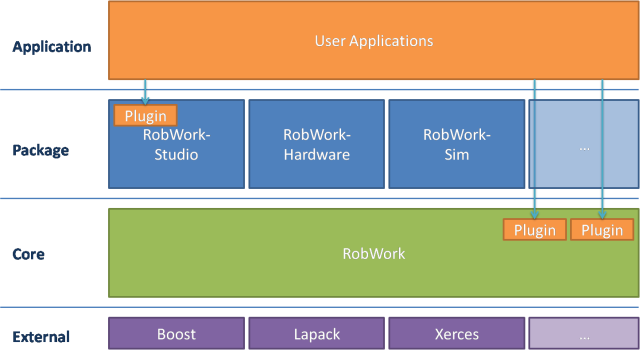
\includegraphics[scale=1]{Figures/RWOverview.png}
	\caption{Overview of the RobWork project \cite{RW_Overview}}
	\label{fig:RWOverview}
\end{figure}